%%%%%%%%%%%%%%%%%%%%%%%%%%%%%%%%%%%%%%%%%%%%%%%%%%%%%%%%%%%
% EPFL report package, main thesis file
% Goal: provide formatting for theses and project reports
% Author: Mathias Payer <mathias.payer@epfl.ch>
%
% To avoid any implication, this template is released into the
% public domain / CC0, whatever is most convenient for the author
% using this template.
%
%%%%%%%%%%%%%%%%%%%%%%%%%%%%%%%%%%%%%%%%%%%%%%%%%%%%%%%%%%%
\documentclass[a4paper,11pt,oneside]{report}
% Options: MScThesis, BScThesis, MScProject, BScProject
\usepackage[MScProject]{EPFLreport}
\usepackage{xspace}

\title{Design and evaluation of mixers\\in a high-churn environment}
\author{Derya Cögendez}
\supervisor{Linus Gasser}
\adviser{Pierluca Borsò-Tan}
%\coadviser{Second Adviser}
\newcommand{\sysname}{FooSystem\xspace}

\begin{document}
\maketitle
\makeacks

\begin{abstract}
Fledger is a peer-to-peer network which works on browsers, it is very modular an can easily be extended with additional services. One of the current services is web proxy module which let's peers act as proxies for other nodes. This service can let \textbf{hide} their traffic patterns from their ISP, however does nothing to protect from traffic analysis by an adversary with limited view of the network nor does it hide traffic patterns from the proxy node. In this project, we do literature review to choose a suitable anonymous communication system for this specific use case of web proxy. We can make crate a proof of concept implementation and tune/evaluate it in the setting of fledger. Given Fledger is a peer to peer network and churn is inevitable, we then add simple mechanisms to improve the reliability of message delivery in the presence of churn. We achieve few seconds latency with \textbf{x percent reliability with these mechanisms}
\end{abstract}

\maketoc

%%%%%%%%%%%%%%%%%%%%%%
\chapter{Introduction}
%%%%%%%%%%%%%%%%%%%%%%
% The introduction is a longer writeup that gently eases the reader into your
% thesis~\cite{dinesh20oakland}. Use the first paragraph to discuss the setting.
% In the second paragraph you can introduce the main challenge that you see.
% The third paragraph lists why related work is insufficient.
% The fourth and fifth paragraphs discuss your approach and why it is needed.
% The sixth paragraph will introduce your thesis statement. Think how you can
% distill the essence of your thesis into a single sentence.
% The seventh paragraph will highlight some of your results
% The eights paragraph discusses your core contribution.

% This section is usually 3-5 pages.
\textbf{Insert something that leads onto fledger without chatgpt speak (something about web proxies maybe)}

Fledger\textbf{cite} is a peer-to-peer network designed to work directly in the browser, without the need for proxies. It enables connecting browsers to communicate between nodes. It is under development and will let users share resources like disk space, CPU, and network bandwidth in the future. Fledger's initial use cases are a decentralized chat application and web proxy. Although with the current version of Fledger, one can use the web proxy, there are some privacy concerns with it. \textbf{insert stuff of isp and traffic analysis} Also, the remote node acting as the web proxy can see all the traffic patterns from the user. 

To remedy this issue we first look into different anonymous communications systems. The first anonymous communication system that comes to mind, Tor\textbf{cite}, is vulrable to traffic analysis [cite stuff].
% To our knowledge there isn't much research into using mixnets for web surfing as for a long time mixnetwork have been limited by their high latency.
% Can probably get some inpiration from one of the mixnet papers
Other communications systems such as .... although solves the problem of Tor, they usually have very high latencies unsuitable for an "instantanous" application such as a web proxy.

We choose Loopix Anonymity System \textbf{cite} for it's low latency, apparent scalability (and tunability) and availability of reference implementations.

We integrate Loopix into Fledger, and adapt it for use for the specific purpose of web browsing through a web proxy. We then choose configuration parameters through extensive experimentation. Although the Loopix paper looks extensively into the privacy aspects of the system, they leave reliable message delivery to future work. \textbf{transition} We explore potential ways to improve the reliability of our implementation. Finally we add simple mechanisms to have more reliable message delivery in the presence of churn.

In conclusion:

% Conclusion: integrated loopix anonymity system into fledger and adapted it for the specific purpose of web proxying with low latency and high reliability. 

%%%%%%%%%%%%%%%%%%%%
\chapter{Background}
%%%%%%%%%%%%%%%%%%%%

% The background section introduces the necessary background to understand your
% work. This is not necessarily related work but technologies and dependencies
% that must be resolved to understand your design and implementation.

% This section is usually 3-5 pages.

\section{Fledger}

Fledger is a P2P network run entirely using browsers, it's goal is to enable user to share resources such as CPU, bandwidth, disk space etc. It uses WebRTC to commnunicate between browsers and uses a Signaling Server to enable nodes to discover each other. Signaling server is currently a centralized component, although in the future the plan is to replace this server with a DHT???

\subsection{Communication between nodes}

\textbf{Talk about web rtc, maybe a figure here.}

When a new fledger node is created it creates a keypair for itself. And from it's public key it derives a nodeID, this nodeID is the main routing information for fledger nodes.

\subsection{Modular Design}

Fledger has a very modular design, for each functionality it has a module that can be enabled within the Fledger node.

Here are the module relevant to this project:
\begin{itemize}
    \item \textbf{Network} \\
    Does all the WebRTC Stuff    
    \item \textbf{Gossip and Random Connections Modules} \\
    Gossip uses Random Connections and Random Connections uses Network module. They are only relevant in this report because we use the gossip module to send all loopix setup information on our experimental setup.
    \item \textbf{Web Proxy} \\
    This module sends and receives web proxy requests, when the module receives a proxy request, it will get the requested website and send it with sections header, body, done in multiple messages.
    \item \textbf{Overlay} \\
    This module acts as a translator/wrapper for fledger modules. While sending a message through gossip of web proxy this module will wrap the message and then send it to the specific module. For example If node A wants to send a web proxy message to node B, web proxy message will be send to overlay module within node A first which will send it to random connections (or network) who will finally the web rtc connection to send the message to node B. Linus Gasser has kindly created this module to help integrate loopix module into Fledger.
    \item \textbf{Loopix} \\
    In this project we have created a loopix module that can be used as a middle man between any module and the network module. The main purpose is to be used with web proxy but it can be used to send other kinds of messages from fledger modules.
\end{itemize}

\section{Loopix Anonymity System}
Loopix is an anonymous communication system that ... It is called a continuous time mixnet as the messages are not delayed between rounds.

\textbf{explain the general idea here}

\subsection{Client}
The users in Loopix are called "clients" these are the nodes that are trying to communicate between each other without being observed.

To achieve this has a send queue. and constantly sends cover traffic.

\subsection{Provider}

Providers in loopix are the entry nodes for the client. Each client has one chosen provider and needs to "subscribe" to this provider. A client will send any message that will go through the mixnet through its provider. If a client receives a message, the provider will store this message and send it to the client only when the client sends a message to retreieve its messages.

\subsection{Mixnodes}

\subsection{Thread Model???}


\subsection{Parameters}
There are many parameters to the Loopix Anonymity System. Which let's us finetune the system to our needs.

\textbf{Talk about how these provide anonymity etc}
\begin{itemize}
\item \textbf{Path Length} \\
How many hops a message goes through the mix network.
\item \textbf{Mean Delay} \\
Mean delay for a messaeg to wait a mixnode.
\item \textbf{Lambda payload} \\
The rate at which the clients sends messages from it's "real" message queue. If it's queue is empty, it will send a dummy\textbf{fact check this} message.
\item \textbf{Lambda loop} \\ 
Rate at which each node sends loop messages \textbf{need to explain loop messages somewhere}. Although the paper separates between the loop rates of mix nodes and clients, for simplicity we use the same thing for all nodes in this project.
\item \textbf{Lambda drop} \\
Rate at which all nodes send drop messages. \textbf{again need to explain drop messages somewhere}
\item \textbf{Time Pull} \\
Rate at which clients asks its provider to send its stored messages. The client always sends this message.
\item \textbf{Max retrieve} \\
The number of messages the provider sends each time it receives a pull request. It always sends this number of messages. If there aren't enough messages for the client, it will send dummy messages to send exactly "max retreieve" number of messages.
\end{itemize}

\subsection{<ean number of messages in the mix}
One important security parameter here is lambda/mu. It is essentially number of messages that are at a mixnode being "mixed" at a time. This is an estimate where lambda is the number of incoming messages every second. And mu is the inverse of the mean delay. One can thing of it as the number of messages that are "leaving" the mixnode on average per second. It is important to note that this estimate assumes that there are no loop messages \textbf{and drop?} being send by the mixnode. The Loopix paper recommends lambda/mu of 2. 


%%%%%%%%%%%%%%%%
\chapter{Design}
%%%%%%%%%%%%%%%%

% Introduce and discuss the design decisions that you made during this project.
% Highlight why individual decisions are important and/or necessary. Discuss
% how the design fits together.

% This section is usually 5-10 pages.

\section{Mix Network Literature Review}

First step in this project was to find a suitable mixer or an anonymous communcation system that can be used in the context of web proxying.

We looked at a multitude of different systems. Here is some of the more relevant ones:

\subsection{Atom}
Development of a scalable anonymous messaging system that defends against traffic analysis attacks. The system is very scalable and techinically over a million users are supports with \textbf{talk about privacy qurantees}, they only achieve 28 minute latency. THis latency might be acceptable for an aync messaging application however, for accessing web pages, this is not usable.

\subsection{Riffle}
Development a bandwidth- and computation-efficient anonymous communication system resistant to traffic analysis. \textbf{talk a bit more about the papers here?} Less than 10 second latency with 100000 users with 100KB/s per user in file sharing applications.  Although 10 seconds is much better than 28 minutes, we are still looking for something that can be more usable for a web proxy. And for the future file sharing applications of fledger 10KB per second would not be enough for a real system.
\subsection{Vuvuzela}
Develop a scalable and flexible metadata-private messaging system that allows asynchronous communication across multiple devices. 37 second latency still not what we are looking for. 
\subsection{Grove}
latency of 32-80 seconds , not enough. Also the focus of the paper was having a an async communicatoin across multiple devices not really latency
\subsection{Prifi}
Low latency DC net with 100ms latency, but only supports up to 100 clients. 

\subsection{Loopix}
As we have talked about Loopix we will not go into further detail here. We chose loopix for it's low latency, scalability, availablility of reference implementations and the tunability of the system. There are also many works that have built on top of loopix which attests to it's extensibility, such as larmix which uses latency aware routing to reduce the network latency between nodes. \textbf{make this a better paraphraph}.

\section{Loopix Integration into Fledger}
\subsection{Loopix as a fledger module}
We we talked about in the background section, fledger contains many modules to communicate between nodes and is very extensible. For this reason we wanted make a loopix module that can fit between any fledger module and the network. Although primary focus of this projec thas been web proxy module, we took care to make sure this module is extensible.

Here is how it works. When a node wants to use web proxy through loopix module, it will create the web proxy module with loopix overlay. Loopix overlay translate the message into a a format that loopix module can understand, note that it could be any fledger module that can send a message to loopix overlay to be translated. Note that only Loopix Clients can send web proxy requests. When loopix module receives a message from overlay it will create a route that goes through its own provider, the mixnetwork, the destion clients provider and finally the client that will be the web proxy. Once the route is created it will create delays for each mixnode. And then encrypt using the public keys of each node. Kind of like onion routing.

Loopix module will then send the encrypted message to network module with the destination as the next node in the route, network module will send it to the destination.

The next node receives the node message in the network module, network module sends the message to loopix module and the loopix module will unwrap one layer from the encryption (provided that it is indeed the correct node that receives the message). This next layer of information contains routing information (only to the next node) as well the specific delay to wait. After waiting the delay, this node sends the message to the network module and so on, until the message eventually reaches the provider of the final destination.

When the provider unpacts the message, it check if the next hop is one of its clients. If so, instead of sending this message directly it stores the message in its own storage until the client asks for messages. When the provider receives a pull request it will send the message along with all the messages in it's storage (it does keep track of the messages it has sent), and if there isn't max retrieve messages to send it will send dummy messages.

Finally the client receives the web proxy request. Through the network module, the network module will peel the final layer of encryption and recover the plaintext, which is a message from the overlay, it will be sent to overlay module, which will in turn translate it into a web proxy message.
\textbf{THE ORIGIN ID IS THERE SO THE PROXY KNOWS WHOS ACCESSING WHICH MESSAGE AGAIN!!!!!!!!!!}
\textbf{BUT this can easily be remedied with the single use reply blocks}

The web proxy module receives the request, gets the url requested and sends all the messages back towards the originator of the request through the network module. And then we go through all the hops again until the provider of the originator etc.

After choosing the mixnet to implement, we integrated fledger into 

\subsection{Assumptions}

\subsection{Bootstrapping}
- signalling server
- nodeID in message
- even unique message ID

\section{Reliable Message Delivery Literature Review}

\section{Adaptations for Reliable Message Delivery and Future Work}

%%%%%%%%%%%%%%%%%%%%%%%%
\chapter{Implementation}
%%%%%%%%%%%%%%%%%%%%%%%%

% The implementation covers some of the implementation details of your project.
% This is not intended to be a low level description of every line of code that
% you wrote but covers the implementation aspects of the projects.l

% This section is usually 3-5 pages.

Some basic details about implementation, no need to talk too much here

talk about parallel message processing

removing storage

using rust sphinx

duplicate messages :)

and there was something else but we'll see

%%%%%%%%%%%%%%%%%%%%
\chapter{Evaluation}
%%%%%%%%%%%%%%%%%%%%

% In the evaluation you convince the reader that your design works as intended.
% Describe the evaluation setup, the designed experiments, and how the
% experiments showcase the individual points you want to prove.

% This section is usually 5-10 pages.

\textbf{PRETTIFY THE GRAPHS AND ADD STD LINES}
\textbf{Talk about what each part in the stacked bar graph represent etc}


\section{Experiental Setup}

\subsection{}
Talk about setup etc and how I wasn't able to setup a massive experiment

number of nodes,
nnetwork latency bandwidth links
nodes operating system cores ram

Experiments where run with 3 clients 6 mix nodes with path length of 3 (2 mixnodes per layer), and 3 providers. With a 50 mbps link between each node with 15ms latency (fully connected). Although in an ideal scenario, this experiment would run with many more nodes with one link connecting to a router node, due to connectivity issues between nodes on the network level as well as lack of documentation in sphere testbed, this has not been possible. However, we still hope to convince the reader of the scalability of the system by the end of this section. 

Each node runs Ubuntu 20.04 LTS with 4 GB RAM and 4 cores on Sphere Testbed \textbf{cite?}. The singal node is running 32 RAM and 32 cores to make sure that it is indeed not a bottleneck.

\textbf{Talk aboout the setup and what thte nodes are doing during the experiment for how long, how many proxy requests over the 5 mins (expect churn stuff)}

\section{Stacked Graph}

\textbf{talk about the different components that contribute to the end to end latency}

\section{Mean number of messages in the mix}
As mentioned in section \textbf{cite section}, one important security parameters for loopix system is the mean number of message in the mix. One issue with the Loopix paper is that in their experiments, they used providers and mixnodes with essentially unlimited resources. \textbf{Quote from the paper here}. Which makes it easy to reach their recommendation of lambda over mu. \\
However, Fledger is designed as a lightweight program, user that want to participate in as mixnode should not need to have \textbf{X amount of RAM and Y cores}. And so keeping in mind that the lambda over mu estimate does not take into account loop messages and the fact that using loopix as already gives up some privacy properties of the original system, we first look into choosing a suitable value for the incoming that a \textbf{low specced machine} can handle.


In this section we keep all parameters of the loopix system stable expect the \textbf{lambda loop drop} etc. This is used to adjust the incoming messages per second while keeping the latency the same, which in turn changes the value of the mean number of message in the mix the mix.

We set mean delay to 100ms which correcsonds to a 1/mu of 1/10, so according to the loopix paper, the target value incoming messages per second is 20. lambda/mu = 2. \textbf{with payload =6?}

\begin{figure}[htbp]
    \centering
    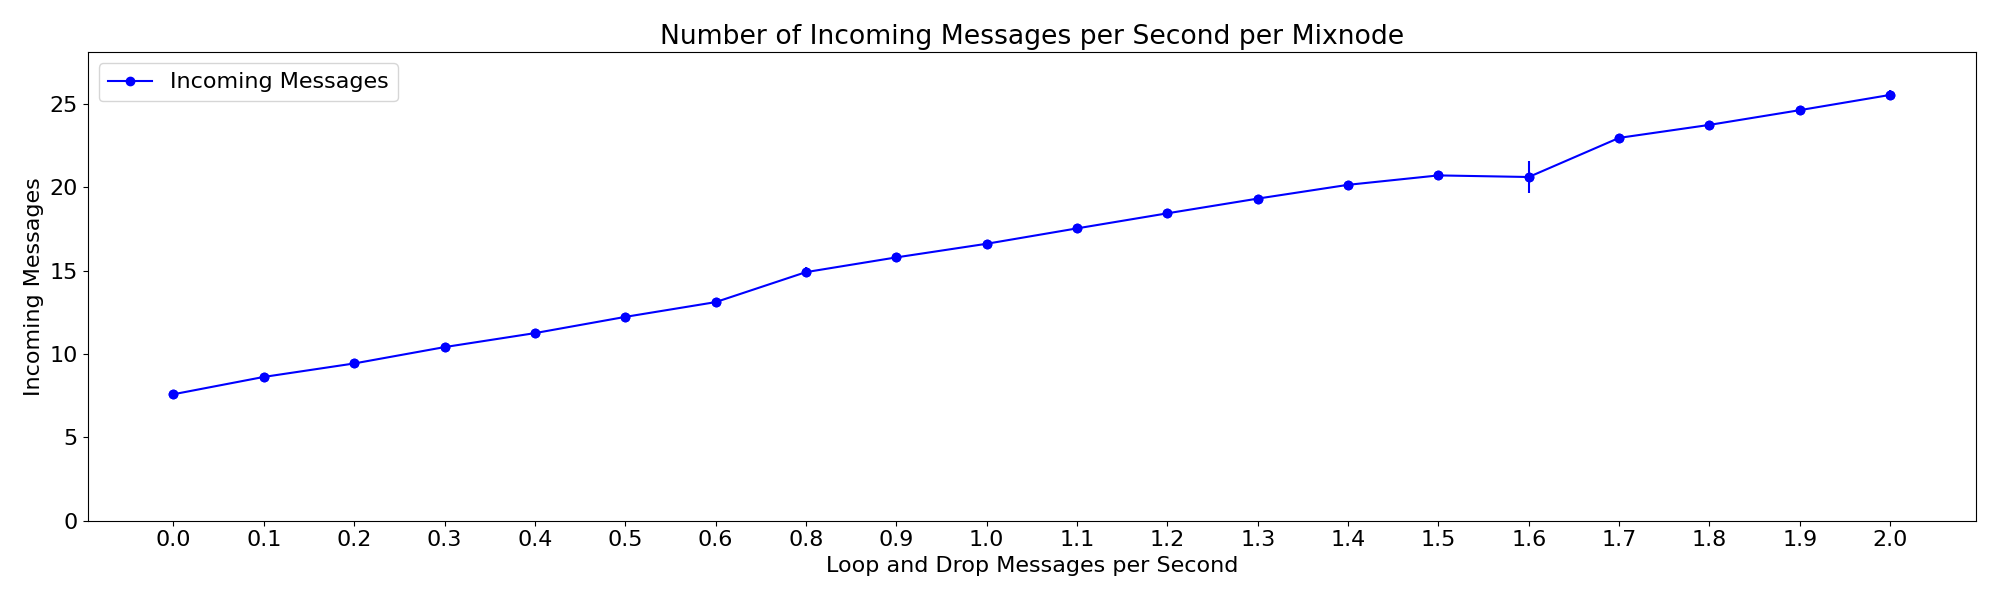
\includegraphics[width=\textwidth]{plots/mu_incoming_messages.png}
    \caption{}
    \label{fig:mu_incoming}
\end{figure}

\begin{figure}[htbp]
    \centering
    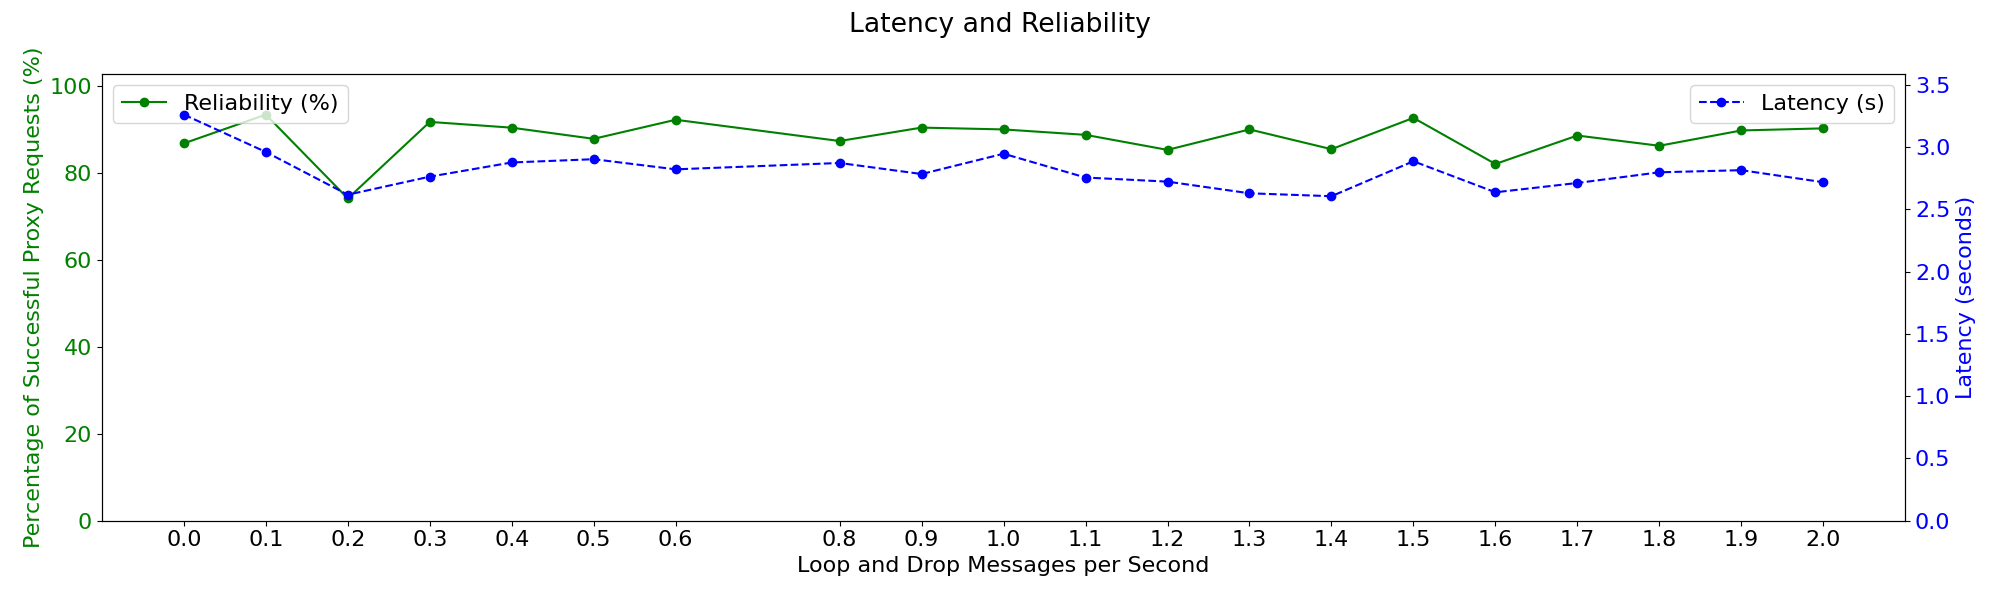
\includegraphics[width=\textwidth]{plots/mu_reliability_latency.png}
    \caption{}
    \label{fig:mu_reliability_latency}
\end{figure}

In \autoref{fig:mu_incoming}, we see that we can adjust the value of the the incoming messages by only adjusting the the cover traffic rates, and in \autoref{fig:mu_reliability_latency}, we see that adjusting the incoming message rate does not affect the reliability the end to end latency of the system.

\textbf{say something about randomness and the measurement is approximate}
This let's us use the recommended lambda/mu value of 2.

\section{Lambda Payload and Mean Delay}
As the most binding limitation in our setup is the end to end latency (a user should be able to surf the internet without waiting too long). In this section try to find lambda payload and mean delay values.

\textbf{Here is how we calculate the lambda over mu values: emprical lol}
\subsection{Lambda payload}

First we adjust the payload value, this warrants a change in the cover traffic rate to keep the mean number of messages one mixnode stable. \textbf{Here we use these values: }





\section{Choosing Max Retrieve and Time pull}

Looking at \textbf{figure X} we can see that provider delay quite a lot.
In this section we choose the max retreive and time pull parameters. essentially, we believe that as we are tuning our system to browse the internet, we do not need to have a very big max retrieve value but the time pull should be low.

\textbf{Talk about how we believe removing/replacing the providers would be beneficial and not retract from the anonymity}

\section{? Why this should work with more nodes}
Although we were not able to set up a experiments with larger number of nodes, in this section we try to demonstrate that our design is scalable:

\section{Reliability Mechanisms}

\subsection{Retry}

\subsection{Duplicate}

\subsection{Combination of Retry and Duplicate}


%%%%%%%%%%%%%%%%%%%%%%
\chapter{Related Work}
%%%%%%%%%%%%%%%%%%%%%%

% The related work section covers closely related work. Here you can highlight
% the related work, how it solved the problem, and why it solved a different
% problem. Do not play down the importance of related work, all of these
% systems have been published and evaluated! Say what is different and how
% you overcome some of the weaknesses of related work by discussing the 
% trade-offs. Stay positive!

% This section is usually 3-5 pages.

Not sure if this section is necessary after all the literature review sections but let's see.

%%%%%%%%%%%%%%%%%%%%
\chapter{Conclusion}
%%%%%%%%%%%%%%%%%%%%

In the conclusion you repeat the main result and finalize the discussion of
your project. Mention the core results and why as well as how your system
advances the status quo.

\cleardoublepage
\phantomsection
\addcontentsline{toc}{chapter}{Bibliography}
\printbibliography

% Appendices are optional
% \appendix
% %%%%%%%%%%%%%%%%%%%%%%%%%%%%%%%%%%%%%%
% \chapter{How to make a transmogrifier}
% %%%%%%%%%%%%%%%%%%%%%%%%%%%%%%%%%%%%%%
%
% In case you ever need an (optional) appendix.
%
% You need the following items:
% \begin{itemize}
% \item A box
% \item Crayons
% \item A self-aware 5-year old
% \end{itemize}

\end{document}